% mainfile: ../../../../master.tex
\subsection{Amplification by PCR with OneTaq\cR polymerase and EMP, \texttt{ARCH} and \texttt{EUK1} primers of DNA extracted extracted with MasterPure\texttrademark~ versus AllPrep kits from micro-algae cultures}
% The part of the label after the colon must match the file name. Otherwise,
% conditional compilation based on task labels does NOT work.
\label{task:20180210_cj0}
\tags{lab,pcr,dna,emp}
\authors{cj}
%\files{}
%\persons{}

\subsubsection{Introduction}
I previously attempted to amplify the two DNA samples to compare the quality of the DNA extracted with the MasterPure\texttrademark~ versus DNA extracted wit the AllPrep kit. The resulting gel did not show strong amplification bands which makes it hard to comclude on which is the best kit to extract DNA. Therefore I am repeating the amplification with some modifications: enhancers and smaller quantities of DNA templates.

\begin{figure}[H] % position of the figure 
    \centering
    \caption{Micro-algae cultures selected (with 'x') for DNA extraction}
    \label{fig:20180207_mia_cultures}
    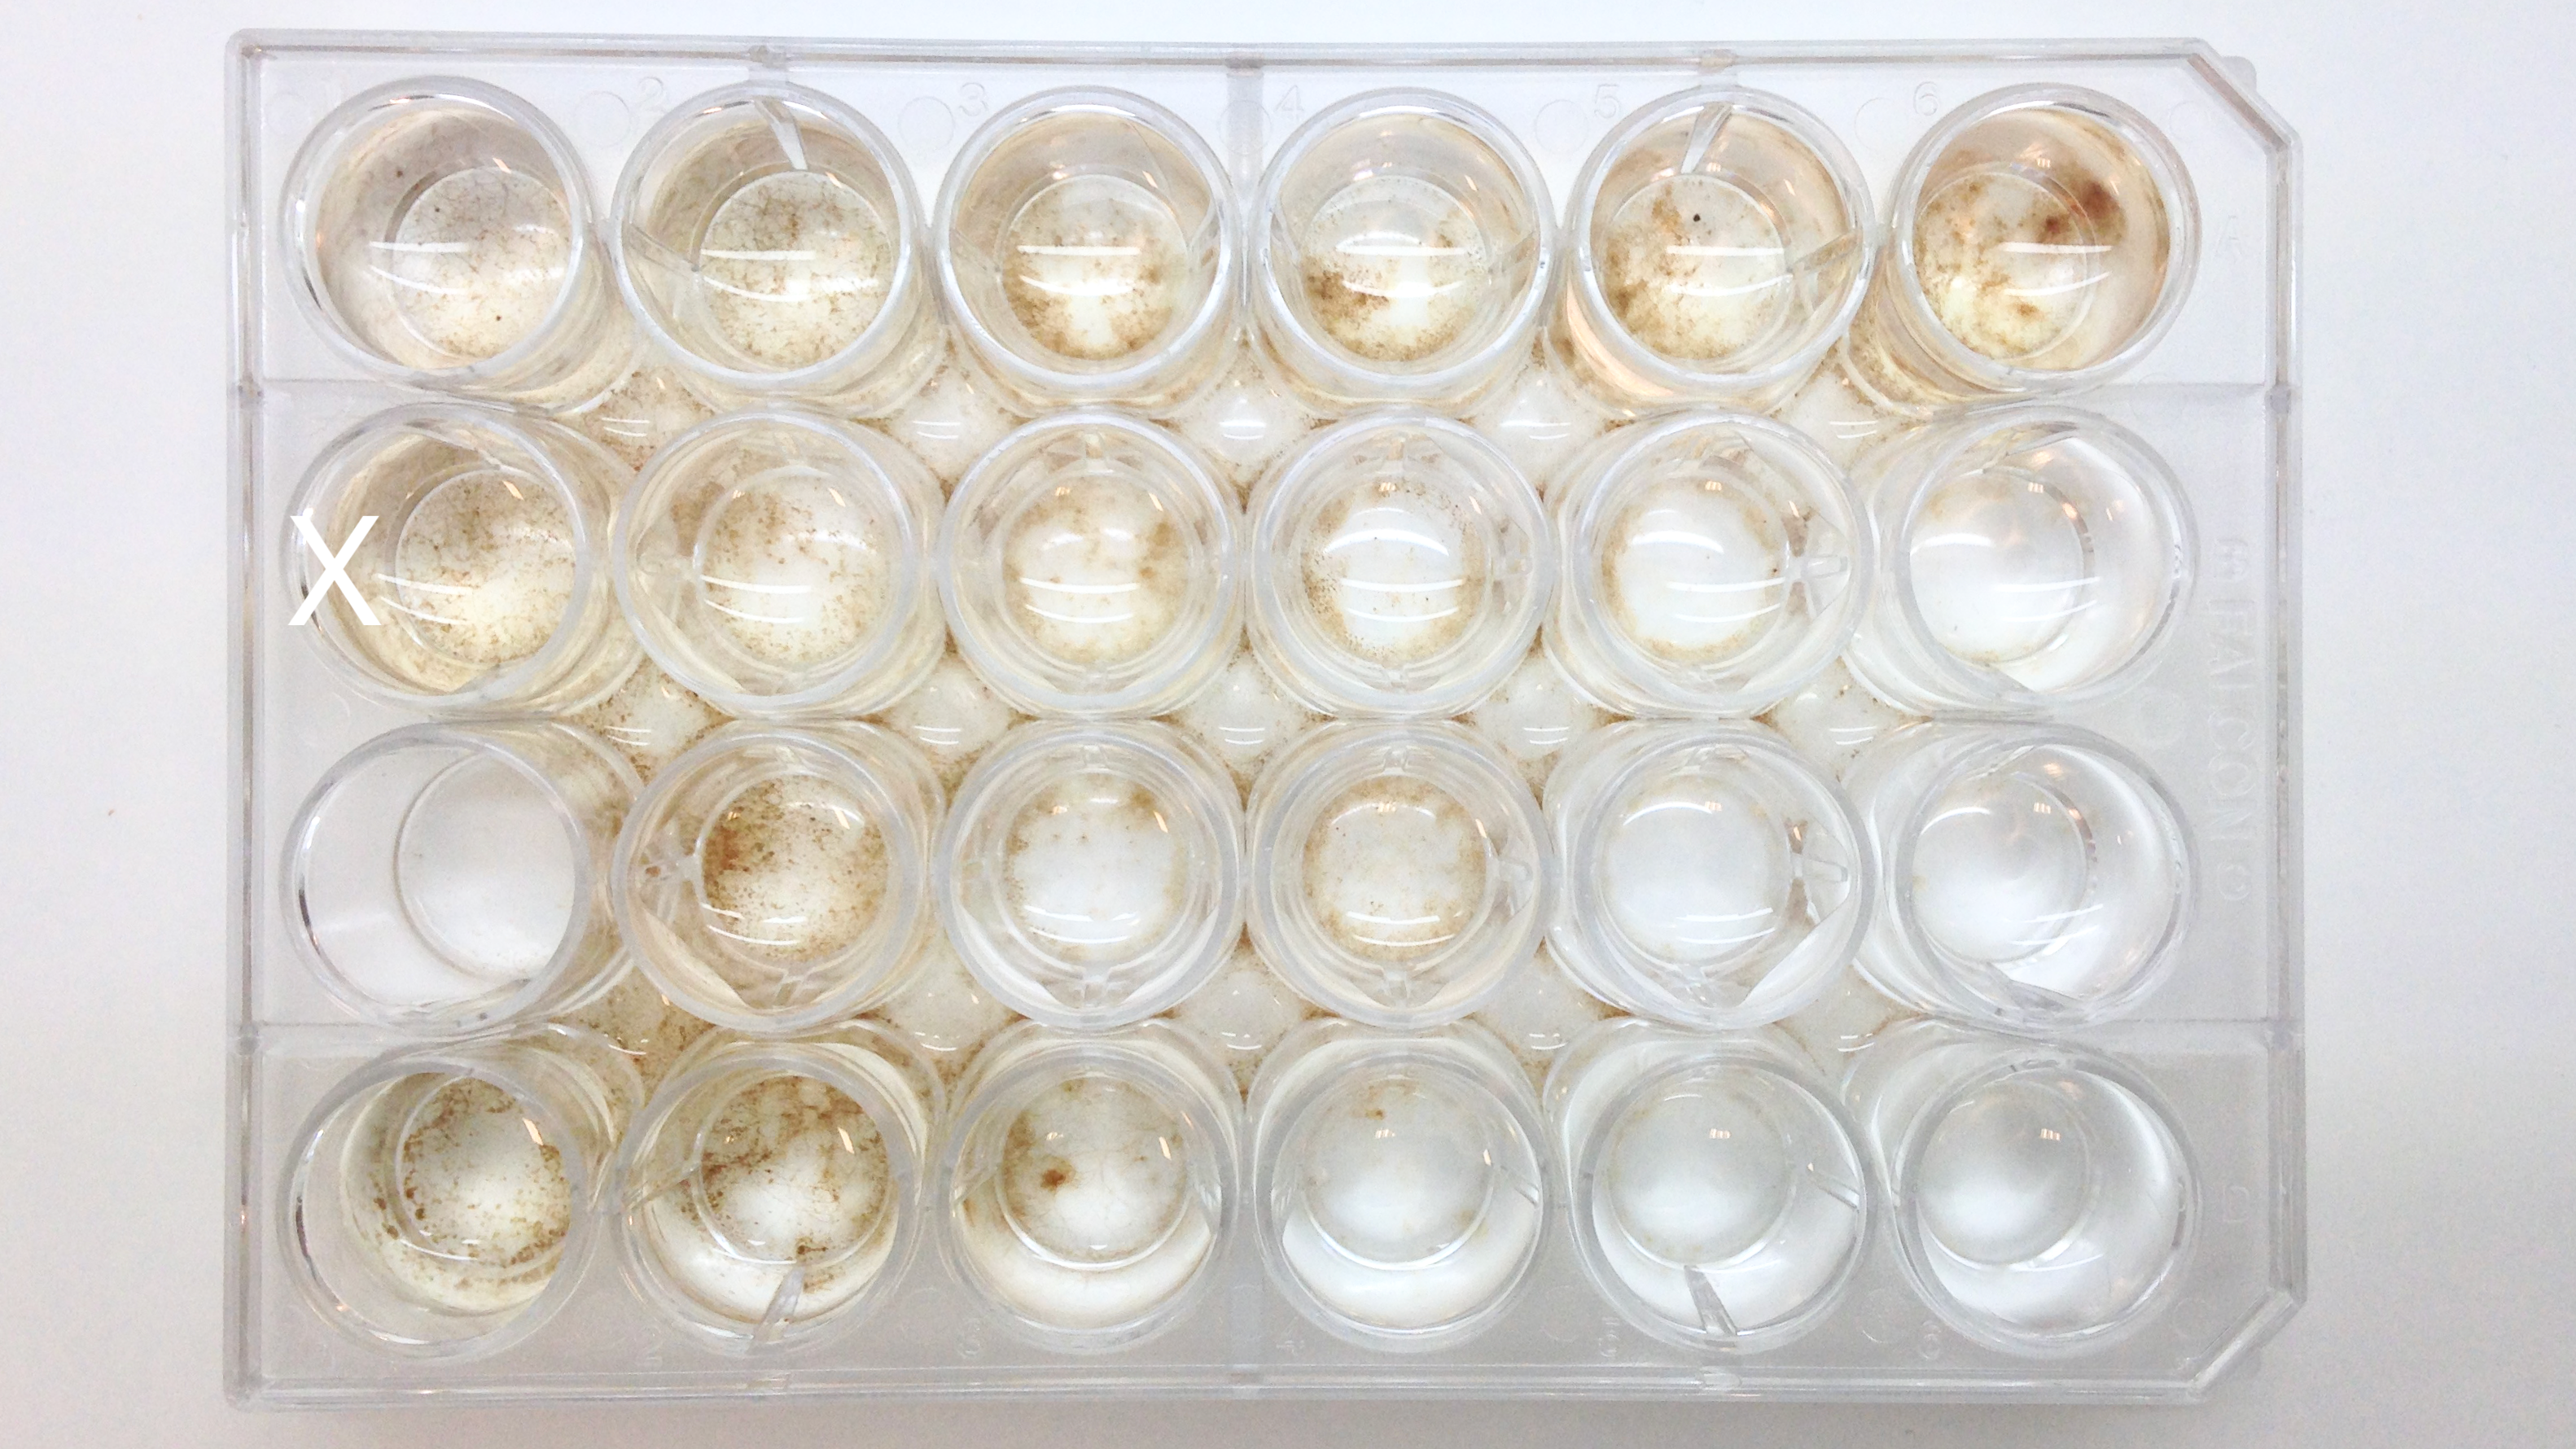
\includegraphics[width=\textwidth]{graphics/pic/20180207_mia_cultures.png}
\end{figure}


\subsubsection{Description of the DNA templates}
\begin{itemize}
\item \texttt{CJ201702} DNA extracted with MasterPure\texttrademark~ from 2~mL of micro-algae culture.
\item \texttt{CJ20170207} DNA extracted with AllPrep kit from 2~mL of micro-algae culture.
\end{itemize}

\subsubsection{Description of controls}
My controls are:
\begin{itemize}
\item[+] diluted DNA from \textit{Thermoanaerobacterium sp.} (Bacteria)
\item[+] DNA from \textit{Thermococcus barophilus} 1 ng/\uL (Archeae)
\item[-] DNA from cod (Eukaryote)
\item[-] Autoclaved MilliQ water
\end{itemize}


\subsubsection{Description of the polymerase}

I will use the \href{https://www.neb.com/products/m0481-onetaq-hot-start-dna-polymerase#Product%20Information}{OneTaq Hot Start DNA polymerase} by New England BioLabs with the \gls{emp} primers.

\subsubsection{Preliminary setup}

\begin{enumerate}
\item Defrost all reagents and samples on ice (1h). \sidenote{It is very important that reagents (especially primers and dNTPs) are fully defrosted otherwise the concentration will not be accurate.}
\item Place all required material in LabCair \gls{pcr} Workstation and turn on \gls{uv} light for at least 20 min.
\end{enumerate}

\subsubsection{Methods}

\begin{enumerate}
\item Work in LabCair \gls{pcr} Workstation
\item Multiply the volume of each reagent by the number of individual \gls{pcr} reactions you wish to perform (including the positive and negative controls) and add 2 extra to account for pipetting error (see table \ref{tab:20180210_mastermix}).
\comment{Today I have 2 samples, 4 controls, and 2 extra, which means I must prepare a master mix for 8 reactions.}
\item In a single 1.5mL-Eppendorf tube combine the following:
	\begin{itemize}
	\item Sterile dH2O
	\item High GC Enhancers
	\item 5X OneTaq Reaction Buffer
	\item dNTP mix (10 mM each nt)
	\item primers
	\item OneTaq\cR Hot Start DNA Polymerase
	\end{itemize}
\item Mix the contents by gently pipetting up and down several times (keep tube on ice)
\item Transfer  15 \textmu L of Master Mix into small \gls{pcr} tubes
\item add 10 \textmu L of \gls{dna} template in each \gls{pcr} tube (on the pre-PCR bench) following the layout shown in figure \ref{tikz:20180210_pcr_racks}.
\comment{I transfer 20~\uL of Master Mix and add 5~\uL of DNA template.}
\item Secure the tops to the \gls{pcr} tubes
\item Tap gently tubes to mix up everything
\item Centrifuge briefly to bring all the liquid to the bottom before placing it in the \gls{pcr} machine
\end{enumerate}

\begin{table}[htbp]
\caption{Master Mix}
\label{tab:20180210_mastermix}
\centering
\begin{tabular}{l r r r r r }
\toprule
Primers & \multicolumn{2}{c}{EMP ARCH} & \multicolumn{2}{c}{EUK1}\\
\cmidrule(l){2-3} \cmidrule(l){4-5} 
 & \multicolumn{2}{c}{Volumes (\uL) for} \\
 \cmidrule(l){2-3}  \cmidrule(l){4-5}
 & 1 reaction & 8 reactions & 1 reaction & 8 reactions \\ 
\midrule 
dH2O & 17.3~\uL & 138.4~\uL & 16.8 & 134.4 \\
High GC Enhancer & 2.5~\uL & 20.0~\uL & 2.5 & 20.0 \\
5X OneTaq Reaction Buffer & 2.5~\uL & 20.0~\uL & 2.5 & 20.0 \\
dNTPs (10mM) & 0.5~\uL & 20.0~\uL & 0.5 & 4.0 \\
Forward primer (10\textmu M) & 0.5~\uL & 4.0~\uL & 0.75 & 6.0 \\
Reverse primer (10\textmu M) & 0.5~\uL & 4.0~\uL & 0.75 & 6.0 \\
OneTaq\cR DNA Polymerase & 0.2~\uL & 1.6~\uL & 0.2 & 1.6 \\
\midrule
Template DNA & 1\uL & - & 1 &  -\\
\midrule
$V_{f}$ (\uL) & 25 &  & 25 & \\
\bottomrule
\end{tabular}
% }
\end{table}

\begin{figure}[htbp]
\caption{Samples organisation in PCR tubes}
\label{tikz:20180210_pcr_racks}
\newcommand*\smp[1]{\texttt{#1}}
\resizebox{\textwidth}{!}{
\begin{tikzpicture}[%remember picture,
  well/.style={rounded rectangle, minimum width=3.5cm, fill=lightgrey, thick, inner sep=3pt, node distance=3pt, minimum height=0.5cm},
  line/.style={fill=white, thick, inner sep=3pt, node distance=3pt, align=left},
  racknum/.style={thick, inner sep=3pt, node distance=3pt, minimum width=0.6cm},
  rack/.style={fill=Aqua, thick, inner sep=3pt, node distance=3pt},
  primer/.style={fill=white, align=left}
  ]
    \node[primer] (emp) {\textbf{EMP}};
       \node[rack, fill=white, below=of emp] (labels1) {
        \begin{tikzpicture}
          \node [racknum, draw=white] (1)  {};
          \node [well, fill=white, right=of 1] (well1)  {A};
          \node [well, fill=white, right=of well1] (well2)  {B};
          \node [well, fill=white, right=of well2] (well3)  {C};
          \node [well, fill=white, right=of well3] (well4)  {D};
          \node [well, fill=white, right=of well4] (well5)  {E};
          \node [well, fill=white, right=of well5] (well6)  {F};
          \node [well, fill=white, right=of well6] (well7)  {G};
          \node [well, fill=white, right=of well7] (well8)  {H};
        \end{tikzpicture}
      };
      \node[rack, below=of labels1] (rack1) {
        \begin{tikzpicture}
          \node [racknum] (1)  {\#~};
          \node [well, right=of 1] (well1)  {\smp{+CTRL ARCH}};
          \node [well, right=of well1] (well2)  {\smp{+CTRL BACT}};
          \node [well, right=of well2] (well3)  {\smp{-CTRL H2O}};
          \node [well, right=of well3] (well4)  {\smp{MP}};
          \node [well, right=of well4] (well5)  {\smp{AP}};
          \node [well, right=of well5] (well6)  {\smp{-Cod}};
          \node [well, right=of well6] (well7)  {\smp{}};
          \node [well, right=of well7] (well8)  {\smp{}};
        \end{tikzpicture}
      };

      \node[primer, below=of rack1] (arch) {\textbf{ARCH}};
       \node[rack, fill=white, below=of arch] (labels2) {
        \begin{tikzpicture}
          \node [racknum, draw=white] (1)  {};
          \node [well, fill=white, right=of 1] (well1)  {A};
          \node [well, fill=white, right=of well1] (well2)  {B};
          \node [well, fill=white, right=of well2] (well3)  {C};
          \node [well, fill=white, right=of well3] (well4)  {D};
          \node [well, fill=white, right=of well4] (well5)  {E};
          \node [well, fill=white, right=of well5] (well6)  {F};
          \node [well, fill=white, right=of well6] (well7)  {G};
          \node [well, fill=white, right=of well7] (well8)  {H};
        \end{tikzpicture}
      };
      \node[rack, below=of labels2] (rack2) {
        \begin{tikzpicture}
          \node [racknum] (1)  {\#~};
          \node [well, right=of 1] (well1)  {\smp{+CTRL ARCH}};
          \node [well, right=of well1] (well2)  {\smp{+CTRL BACT}};
          \node [well, right=of well2] (well3)  {\smp{-CTRL H2O}};
          \node [well, right=of well3] (well4)  {\smp{MP}};
          \node [well, right=of well4] (well5)  {\smp{AP}};
          \node [well, right=of well5] (well6)  {\smp{-Cod}};
          \node [well, right=of well6] (well7)  {\smp{}};
          \node [well, right=of well7] (well8)  {\smp{}};
        \end{tikzpicture}
      };
      
      \node[primer, below=of labels2] (euk1) {\textbf{EUK1}};
       \node[rack, fill=white, below=of euk1] (labels3) {
        \begin{tikzpicture}
          \node [racknum, draw=white] (1)  {};
          \node [well, fill=white, right=of 1] (well1)  {A};
          \node [well, fill=white, right=of well1] (well2)  {B};
          \node [well, fill=white, right=of well2] (well3)  {C};
          \node [well, fill=white, right=of well3] (well4)  {D};
          \node [well, fill=white, right=of well4] (well5)  {E};
          \node [well, fill=white, right=of well5] (well6)  {F};
          \node [well, fill=white, right=of well6] (well7)  {G};
          \node [well, fill=white, right=of well7] (well8)  {H};
        \end{tikzpicture}
      };
      \node[rack, below=of labels3] (rack3) {
        \begin{tikzpicture}
          \node [racknum] (1)  {\#~};
          \node [well, right=of 1] (well1)  {\smp{}};
          \node [well, right=of well1] (well2)  {\smp{+Cod}};
          \node [well, right=of well2] (well3)  {\smp{-BACT}};
          \node [well, right=of well3] (well4)  {\smp{-ARCH}};
          \node [well, right=of well4] (well5)  {\smp{-dH2O}};
          \node [well, right=of well5] (well6)  {\smp{MP}};
          \node [well, right=of well6] (well7)  {\smp{AP}};
          \node [well, right=of well7] (well8)  {\smp{}};
        \end{tikzpicture}
      };
\end{tikzpicture}
}

\end{figure}

\begin{table}[htbp]
\caption{Thermocycler settings}
\label{tab:20180210_thermocycler_settings}
\centering
\begin{tabular}{l r r}
 & \multicolumn{2}{c}{\texttt{EMP} \& \texttt{ARCH}}\\
\cmidrule(l){2-3}
Steps & T(\degree C) & Time \\
\midrule
Initial denaturation & 94 & 30 sec \\
\midrule
Denaturation & 94 & 30 sec \\
Annealing & 50 & 40 sec \\
Extension & 68 & 30 sec \\
\midrule
Final extension & 68 & 5 min \\
Infinite hold & 4 & - \\
\bottomrule
\end{tabular}
% }
\end{table}
